\documentclass[a4paper, doc, natbib]{apa7}
\usepackage[utf8]{inputenc}
\usepackage[english]{babel}
\usepackage{amsfonts}
\usepackage{amssymb}
\usepackage{amsmath}
\usepackage{amsthm}
\usepackage{graphicx}
\usepackage{natbib}
\usepackage{txfonts}
\usepackage{multirow}
\usepackage{mathtools}
\usepackage{subcaption}
\usepackage{tabularx}
\usepackage{setspace}
\doublespacing

\bibliographystyle{apalike}

\title{State of the art time series models in JASP: Development of a Bayesian state space module}
\shorttitle{Bayesian structural time series in JASP}
\author{Fridtjof Petersen}
\affiliation{University of Amsterdam}
\date{\today}
\authornote{E-mail: fridtjof.petersen@student.uva.nl}
\begin{document}

\maketitle



\section{Introduction}
Let us consider two time series problems: In March 2021 NASA managed to land its rover on mars. But how was it possible to track and forecast/predict a spacecraft’s true location in space when we only have our imprecise sensor measurements? Or we have a previously depressed patient whose depression status is monitored through daily questionnaires and wonder: Can we identify the factors influencing his depression and predict whether his condition will worsen? In both problems we want to monitor and estimate a process over time and make a forecast about its future behaviour.

One popular and flexible solution to this problem are state space models: State space models describe the dependence between hidden states $\alpha_t$ containing our parameter of interest and our actual observations $y_t$. The states $\alpha_t$ are Markov chains as they only depend on their previous iteration $\alpha_{t-1}$ and our observations $y_t$ only on the corresponding state. Applied to our examples at the beginning, our hidden states would be the true depression or the exact location in space while we can only observe the questionnaire or sensor measurements. One of the most popular tools to estimate these states is the Kalman Filter \citep[for a Bayesian derivation see:][]{meinholdUnderstandingKalmanFilter1983,petrisDynamicLinearModels2009} which is recursive in nature: It combines the previous state estimate with the current observation to obtain the best estimate for the current state. This allows us to seamlessly integrate new data into our model as we only need the previous state estimate and our current observation. 

State space models offer great flexibility as the state space notation is modular in nature which allows us to include various processes  (Durbin & Koopman, 2012). This means that the state vector can contain multiple components such as autoregressive processes, seasonality or even regression coefficients. Thus state space models can represent a wide variety of traditional models ranging from static regression models to all AR(I)MA models, which is elaborated in the method section. While it is also possible to model non-linear and non Gaussian processes with state space models (see Durbin & Koopman, 2012), the current paper will focus on linear gaussian (i.e. normal) processes as described by Scott and Varian (2014, 2015). Their Bayesian structural time series takes the classical state space model and extends it with Bayesian variable selection and model averaging (George & McCulloch, 1997). 

The Bayesian nature of the BSTS model has the advantage of providing us with a posterior distribution for both our time series as well as our regression coefficients. This becomes important when we want to identify the most important predictors: If we use only the most fitting model, we might lose information that all the discarded yet less probable ones possess. Bayesian model averaging on the other hand averages over all possible models and gives them different weights depending on how probable they are (Hinne et al., 2020). 

Despite the flexibility and generality of state space models, they only have found scarce applications in the social sciences (some examples Chow et al., 2009; Hamaker & Grasman, 2012; Lodewyckx et al., 2011; Molenaar et al., 2009). As a reason for this it has been noted that social science researchers are often unfamiliar with their notation. Furthermore, the existing implementations require researchers to know how to program and properly apply state space models. This highlights the need for an implementation that is easy to use so more social science researchers can benefit from state space models.

In hopes of easing accessibility to the benefits of the BSTS model, the following paper will outline the BSTS model and introduce an implementation of the bsts R package by Scott and Varian (2014) in the statistical program JASP (JASP Team, 2020). JASP is free, open source and has a user friendly interface which allows easy access to both Bayesian and frequentist analysis.

The benefit of the state space model may become more apparent if we compare it to the classical way of fitting time series data in the social sciences: The classical autoregressive (AR)  model captures temporal dependencies by predicting the current observation from previous observations via an autoregressive coefficient  (Hamilton, 1994). One more flexible extension of the AR model is the time varying autoregressive model where the intercept and autoregressive coefficients are allowed to vary over time: Here the model is fitted with smoothing splines from generalised additive models \citep{bringmannChangingDynamicsTimevarying2017,woodGeneralizedAdditiveModels2017} which allows the parameters to vary without having to specify the form of change beforehand.

Yet one major drawback of fitting the classic time varying AR models is that they can only be fitted offline - which means only after we have collected all and enough data. Inference for the time varying AR model is usually done in a frequentist framework we are unable to fit the model again and again as we receive data without increasing our false positive error rate. Furthermore, in order to fit time varying AR models by regression splines, cross validation is necessary to achieve a balance between fit and smoothness of the splines. This requires a rather large sample that has to be collected prior to estimation due to the cross validation method used (Bringmann et al., 2017; Wood, 2017). Yet state space models allow us to create estimate our model from the first observation onwards while being able to integrate new observation seamlessly (Durbin & Koopman, 2012). 



\section{Method}
Before we dive into the specific parts and functions of the module, let's revisit the state space model in more detail: The state space model describes how our process develops over time by linking the hidden/latent states $\alpha_t$ with the observed values $y_t$ \citep{durbinTimeSeriesAnalysis2012}. As the states $\alpha_t$ are Markov chains they only depend on the previous iteration $\alpha_{t-1}$ while the observations are only depend on the state which is shown in figure 1. 


\begin{figure}
    \centering
    \caption{This is my first figure caption.}
    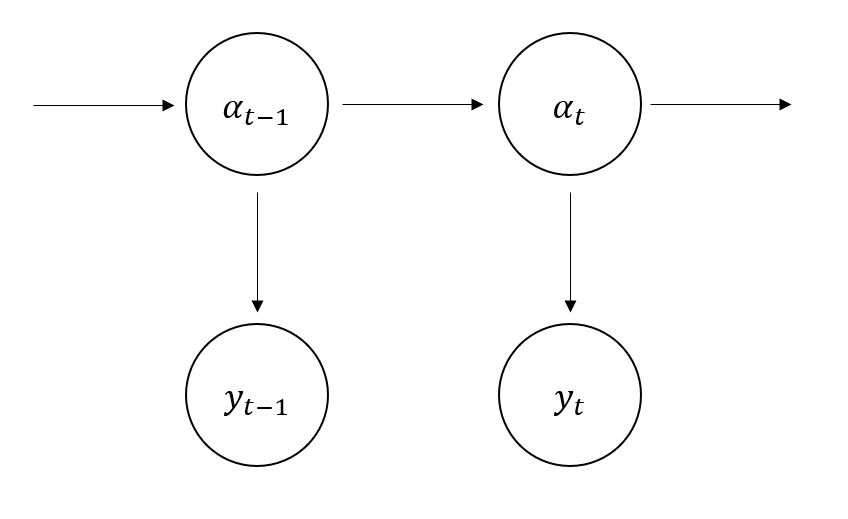
\includegraphics[scale=0.7]{state.pdf}
    \label{fig:Figure1}
\end{figure}


These two characteristics of state space models are formally described by two equations. The  first one is the state equation:

$$
\alpha_{t} = T_t^T \alpha_{t-1} + \eta_t \quad \eta_t \sim \mathcal{N}(0,Q_t) \quad \quad(1)
$$
Here, the \textit{state vector} $\alpha_t$ may contain all variables that we are interested in such as slope, (auto)regressive coefficients or seasonal components \citep{scottPredictingPresentBayesian2014}. The transition matrix $T_t$ tells us how our current state evolved from the previous one, and the error term $\eta_t$ is a the Gaussian process noise with a mean of 0 and the variance (matrix) $Q_t$. 
The second equation needed is the \textit{transition} or \textit{observation equation} which relates our hidden states to the observations,
$$
y_{t} = Z_t^T \alpha_{t} + \epsilon_t \quad \epsilon_t \sim \mathcal{N}(0,H_t) \quad \quad(2)
$$
as the matrix $Z_t$ determines how our state vector impacts our observation vector $y_t$. The error term $\epsilon_t$ is our measurement error and also has a Gaussian distribution with a mean 0 and variance $H_t$. (maybe include that error terms modelled separately which is nice).

When models are written in the form of equation (1) and (2) they are said to be in sttae space form. The model described here is the linear Gaussian case as this can be fitted with the Kalman filter. The benefit of the linear version is that components of the state vector can simply be added to each other which makes their estimation computationally efficient\citep{fangNonlinearBayesianEstimation2017}. If these assumptions are not met however, methods such as the extended Kalman Filter or non-parametric methods like particle filters are available (for an overview see: Fang et al.,2017.

The Kalman filter is of an Bayesian nature as we arrive at a probability distribution for our states. This simplifies using the Markov Chain Monte Carlo method to sample from the posterior distribution to perform Bayesian inference. Furthermore this allows us to integrate any prior beliefs we have about each state component. 

One attractive feature of the BSTS model is variable selection and model averaging which will be briefly described \cite[see an extensive explanation see][]{scottPredictingPresentBayesian2014,scottBayesianVariableSelection2015} : In order to select the optimal number of predictors, each possible regression coefficient is assigned a so called spike-and-slab prior. The spike prior refers to the probability of each regression coefficient being zero or not while the slab prior quantifies the size of each regression coefficient given that is not zero. After applying the MCMC we get a posterior distribution of inclusion probability and the corresponding value for the coefficient. The model averaging averages over all possible combinations of predictors and give them weight according to their probability. This allows us to retain information that we would have lost if we would have used the best fitting model.

\subsection{The building block of the JASP module: The bsts package}

In the following the future functions of the JASP module will be based in more detail. They are based on the \textit{bsts} package \citep{scottBstsBayesianStructural2020} in the statistical software R\citep{rcoreteamLanguageEnvironmentStatistical2021}. First, one specifies the components of the state vector and afterwards estimates their distribution and samples from it. 

The first state specification to be included will be the \textit{autoregressive model} from the \textit{AddAr} function. Here the current state $\alpha_t$ is connected to the selected lagged states $\alpha_{t-p}$ via a autoregression coefficient $\phi_{t-p}$. An extension to this the \textit{AutoAR} function, which, similar to the regression component, places a spike-and-slab prior to all selected regression coefficients and gives an indication about which lags to include.

The \textit{local level model} component is added via the \textit{AddLocalLevel} function where the state evolution is only described by a level (or intercept) $\mu_t$ following a random walk. As an extension to this the \textit{AddLocalLinearTrend} function adds an additional slope component $v_t$  to the level $\mu_t$ that also follows a random walk. In contrast the \textit{addSemiLocalLinearTrend} function adds a local linear trend component the trend component $v_t$ follows an autoregressive process with a lag of 1, which might be more appropriate for forecasting. 

If one has extensive time series data, it might also be sensible to include a seasonal component, which captures reoccurring and systematic changes in the state. This will be included with the \textit{AddSeasonal} function where one can choose the number of seasons and the duration of each season. This adds a dummy variable for each season to the state specification. It will be possible to add multiple seasonal components as one could suspect weekly, daily and hour-of-the-day patterns. 

The JASP module will also include the possibility to include regression coefficients which can either be dynamic or static. A table regarding the regression coefficients' size and inclusion probability will be provided as well as a plot to visualise this. 

All of the aforementioned components will be combined via the \textit{bsts} function: It applies the Kalman filter which estimates the state and uses the MCMC to sample from the posterior distribution of all state components. It will be possible to plot the posterior distribution of the state against the actual observations as well as the contribution of each individual state component. Furthermore it will be possible to predict future observations. 

As the focus of this project is purely on developing a state space module in JASP, no data collection or large simulations will be conducted. However in order to verify the functionality of the developed module, a mix of simulated and already existing data sets will be analysed and reported upon. 



 





\vspace{5mm}
\noindent

\section{Work plan}
\noindent



\begin{tabularx}{0.8\textwidth} { 
  | >{\raggedright\arraybackslash}X 
  | >{\centering\arraybackslash}X|}
 \hline
 Internship duration & 01-03-2021 - 26-06-2021 \\
 \hline
 Number of EC & 18 \\
 \hline
 Number of weeks  & 21 \\
\hline
 Time investment in hours per week & 24 \\
\hline
\end{tabularx}



\begin{tabularx}{0.9\textwidth} { 
  | >{\raggedright\arraybackslash}X 
  | >{\centering\arraybackslash}X|}
 \hline
 Submission of the Internship proposal to peer-review & 04/03/2021 \\
\hline
 Developing a general interface for the JASP module & 05/03/2021 - 11-/04/2021 \\
\hline
 Implementing the individual state components & 12/04/2021 - 02/05/2021 \\
\hline
 Analysing exemplary real and simulated data & 03/05/2021- 16/05/2021 \\
\hline
 Writing documentation for the module&  10/05/2021 - 30/05/2021 \\
\hline
 Writing the internship report & 31-05-2021 - 25-06-2021 \\
\hline
\end{tabularx}



\bibliography{ref}

\end{document}
